\section{Implementation Overview}
This section will give an overview of the different components and the overall flow of \pyt{}.
An illustration giving an abstract overview can be seen on \cref{figure:implementation_overview}.

\begin{figure}
  \begin{tikzpicture}
\newcommand\XLabel{7}
\newcommand\XNode{10}
\newcommand\XEngines{14}
\newcommand\TextWidth{3}
\tikzset{>=latex}

%\draw[help lines] (5,5) grid (15,20);

%%%%%%%%%%%% MID STRUCTURE %%%%%%%%%%%%%%%%%%%
\node[inner sep=10pt] (code) at (\XNode,18)
    {
\includegraphics[width=.1\textwidth]{./figures/dot_files/implementation_overview_images/source_code.png}};
\node[text width=\TextWidth{}cm] at (\XLabel,18) {\hfill{}Source code};

\node[inner sep=10pt] (ast) at (\XNode,15)
    {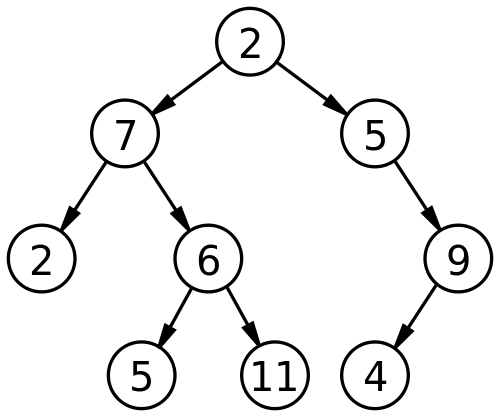
\includegraphics[width=.15\textwidth]{./figures/dot_files/implementation_overview_images/ast.png}};
\node[text width=\TextWidth{}cm] at (\XLabel,15) {\hfill{}AST};

\node[inner sep=10pt] (cfg) at (\XNode,11)
    {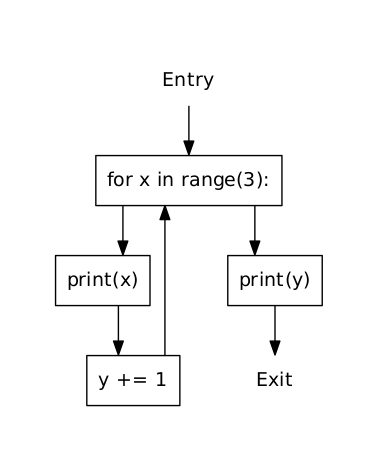
\includegraphics[width=.2\textwidth]{./figures/dot_files/implementation_overview_images/for_complete.png}};
\node[text width=\TextWidth{}cm] at (\XLabel,11) {\hfill{}CFG};

\node[inner sep=10pt] (engine) at (\XNode,7)
    {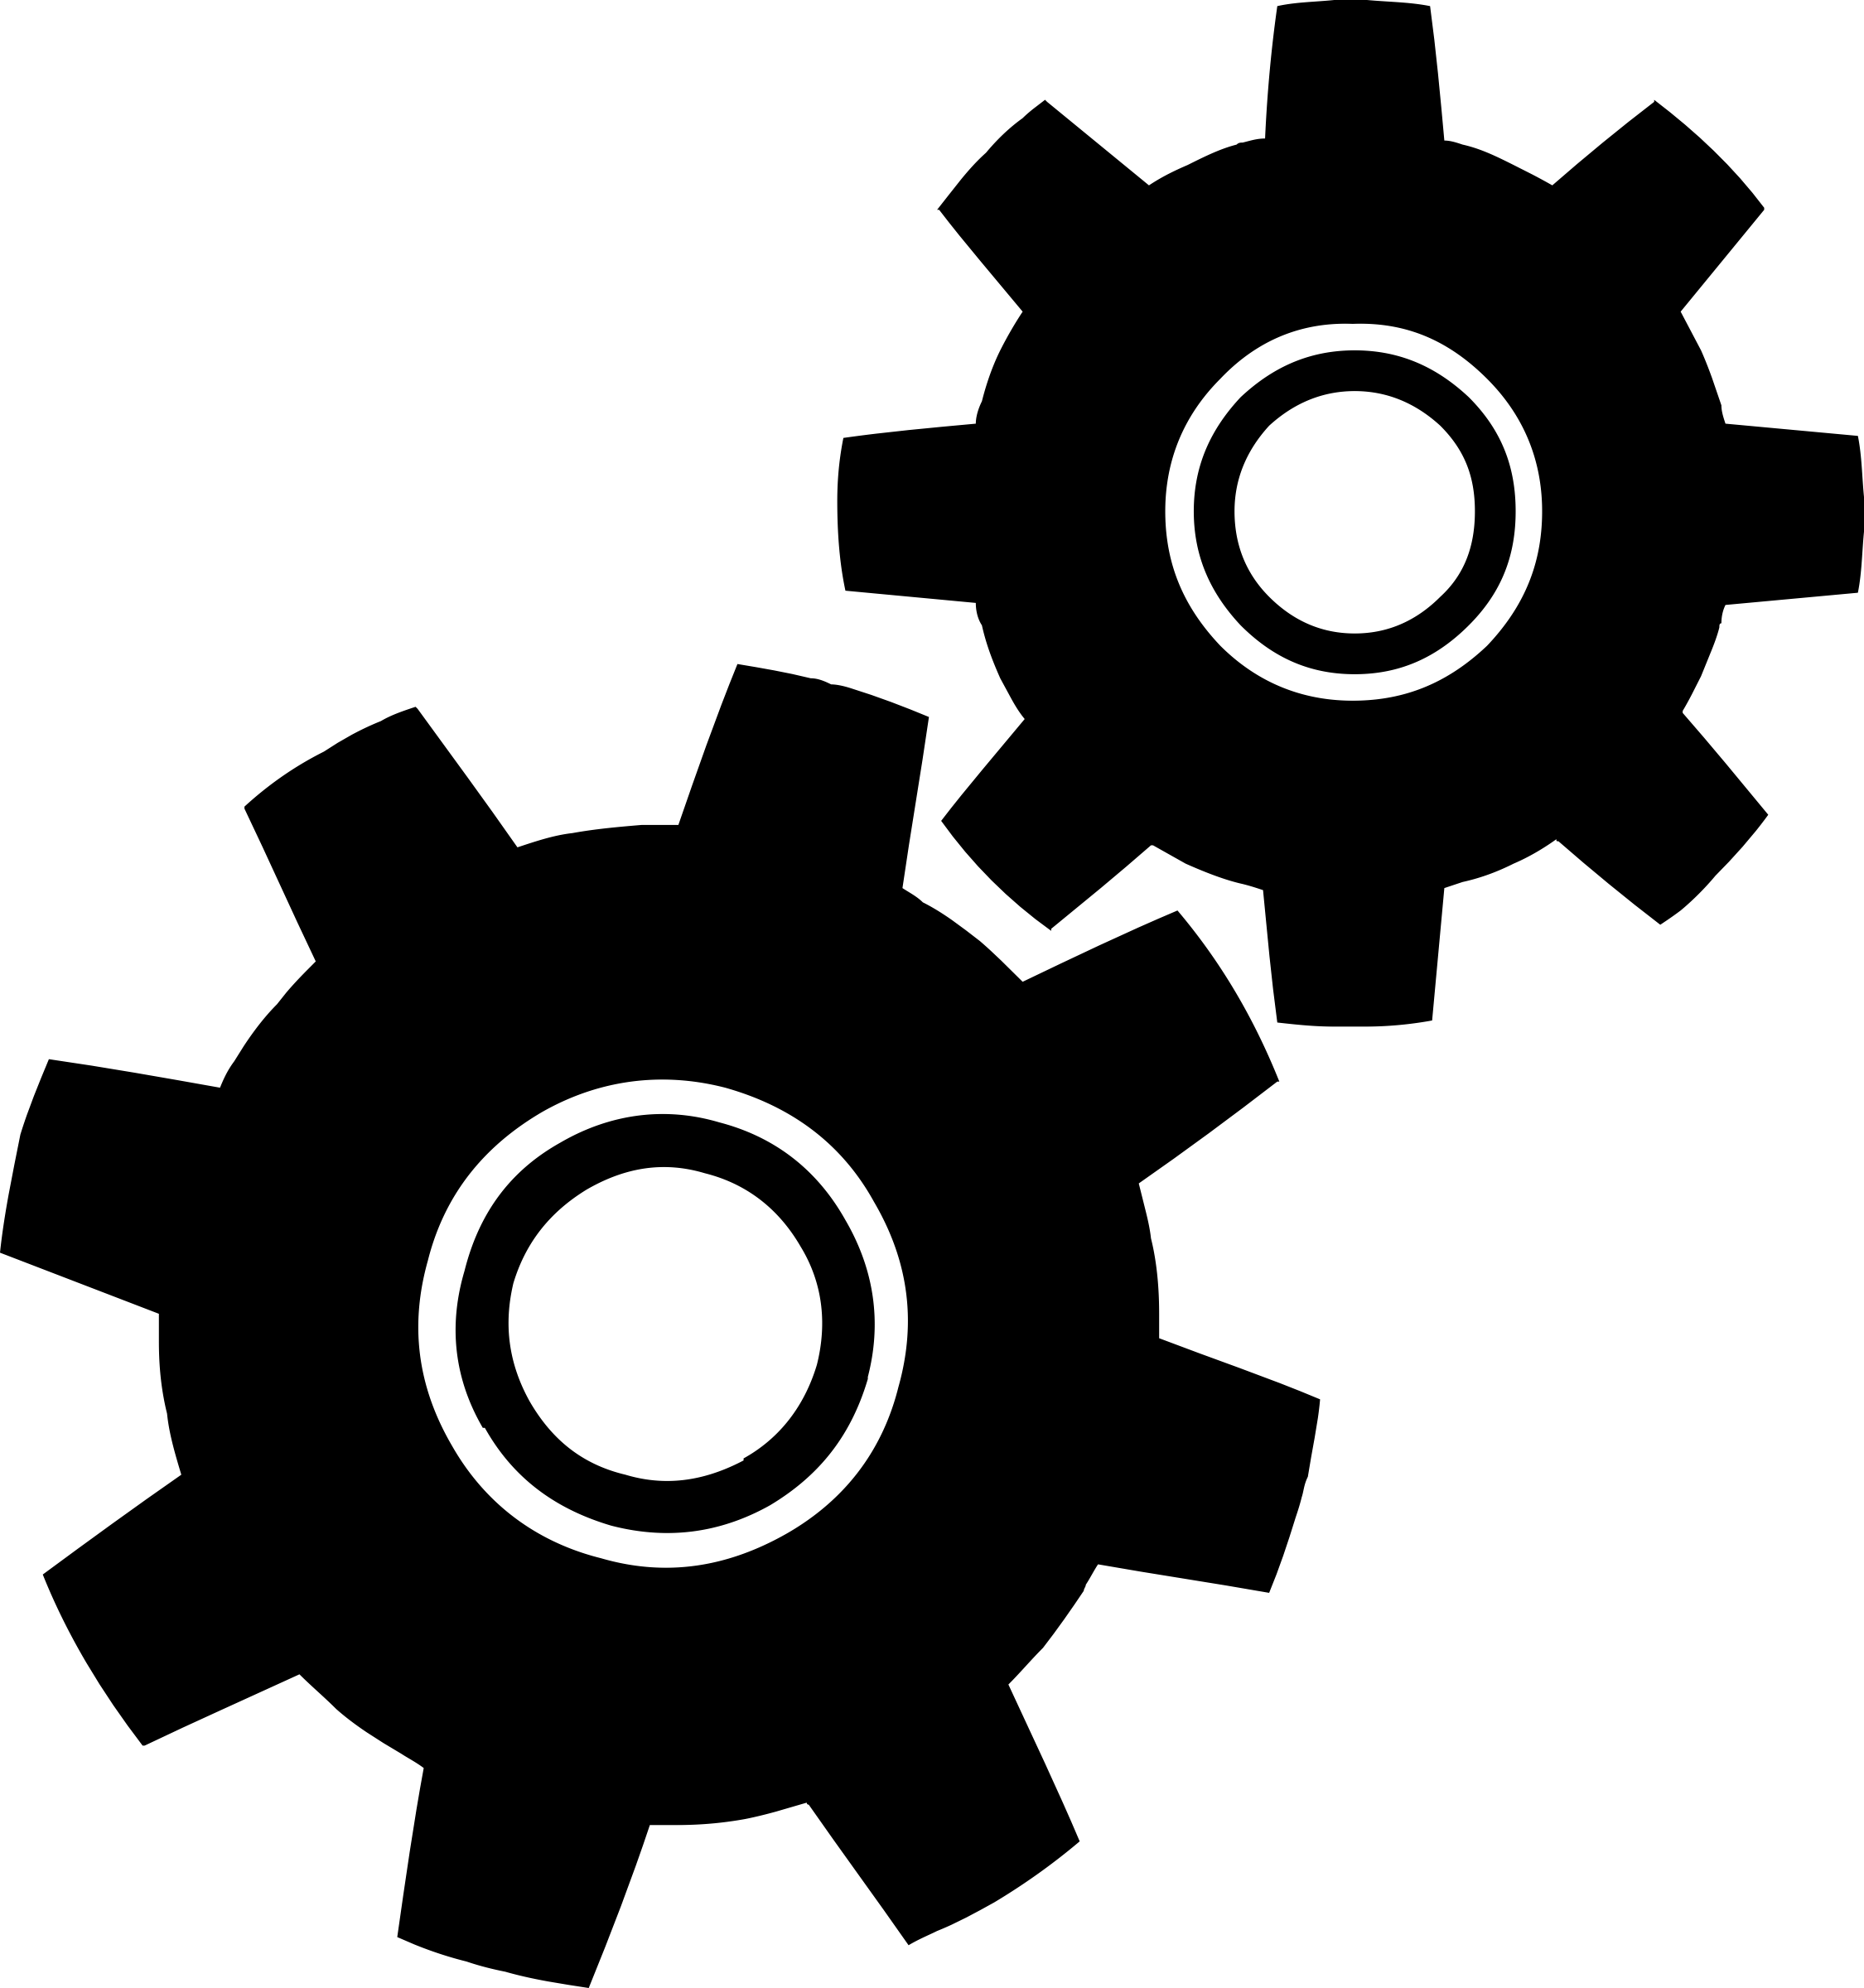
\includegraphics[width=.1\textwidth]{./figures/dot_files/implementation_overview_images/cog_wheel.png}};
\node[text width=\TextWidth{}cm] at (\XLabel,7) {\hfill{}Engine};

\node[inner sep=10pt] (algorithm) at (\XNode,4)
    {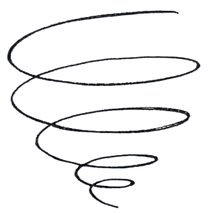
\includegraphics[width=.1\textwidth]{./figures/dot_files/implementation_overview_images/spiral.png}};
\node[text width=\TextWidth{}cm] at (\XLabel,4) {\hfill{}Fixed Point \\ \hfill{}Algorithm};

\node[inner sep=10pt] (vulnerabilities) at (\XNode,1)
    {
\includegraphics[width=.15\textwidth]{./figures/dot_files/implementation_overview_images/vulnerability.png}};
\node[text width=\TextWidth{}cm] at (\XLabel,1) {\hfill{}Vulnerabilities};

%%%%%%%%%%%%%%%%%%%% ENGINES %%%%%%%%%%%%%%%%%%%%%%%%
\node[inner sep=10pt] (flask) at (\XEngines,11)
    {
\includegraphics[width=.2\textwidth]{./figures/dot_files/implementation_overview_images/flask_text.png}};

\node[inner sep=5pt] (django) at (\XEngines,9)
    {
\includegraphics[width=.13\textwidth]{./figures/dot_files/implementation_overview_images/django.png}};

\node[label=below:{Other}, inner sep=5pt] (other_engine) at (\XEngines,7)
    {
\includegraphics[width=.05\textwidth]{./figures/dot_files/implementation_overview_images/question_mark.png}};

%%%%%%%%%%%%%%%% ANALYSIS %%%%%%%%%%%%%%%%%%%%%%%%%    
\node[label=below:{Analysis}, inner sep=10pt] (analysis) at (\XEngines,4)
    {
\includegraphics[width=.1\textwidth]{./figures/dot_files/implementation_overview_images/analysis.png}};

\node[text width=2cm, inner sep=10pt] (reaching) at (18,7) {Reaching Definitions};
\node[text width=2cm, inner sep=10pt] (liveness) at (18,4) {Liveness};

\node[label=below:{Other}, inner sep=5pt] (other_analysis) at (18,1)
    {
\includegraphics[width=.05\textwidth]{./figures/dot_files/implementation_overview_images/question_mark.png}};


\draw[->] (code) -- (ast);
\draw[->] (ast) -- (cfg);
\draw[->] (cfg) -- (engine);
\draw[->] (engine) -- (algorithm);
\draw[->] (algorithm) -- (vulnerabilities);

\draw[->] (flask) -- (engine);
\draw[->] (django) -- (engine);
\draw[->] (other_engine) -- (engine);

\draw[<->] (algorithm) -- (analysis);
\draw[->] (reaching) -- (analysis);
\draw[->] (liveness) -- (analysis);
\draw[->] (other_analysis) -- (analysis);

\end{tikzpicture}
  \caption{An abstract overview of the implementation of \pyt{}, showing the main components and the flow.}
  \label{figure:implementation_overview}
\end{figure}

The illustration shows that \pyt{} takes some source code as input and outputs at last a list of potential vulnerabilities.
After the source code is loaded an abstract syntax tree(AST) is generated.
The AST is generated using the standard Python library \texttt{ast}\cite{python_ast}.
One of the biggest components is the CFG component, which uses the AST nodes to make CFG nodes.
The engine is a component that uses a defined engine to prepare the CFG on the analysis.
The default engine is the Flask engine.
The fixed point algorithm is basically just implemented as the algorithm is described in \cref{fixed_point_algorithm}.
But it is able to use different analyses and as default it uses the reaching definitions analysis.
These analyses can be specified by the user.
At last a vulnerability log is provided to the user giving precise information about the potential vulnerabilities found.
